\documentclass[a4paper,10pt]{article}

\usepackage{fullpage}
\usepackage[T1]{fontenc}
\usepackage{graphicx}
\usepackage{float}
\usepackage{amsmath}
\usepackage{tabulary}
\usepackage{listings}
\usepackage[spanish]{babel}
\usepackage[utf8]{inputenc}
\usepackage{color}
\usepackage[pdfborder={0 0 0}]{hyperref}
\usepackage{alltt}
\usepackage{moreverb}
\usepackage{enumitem}
\usepackage{array}
\usepackage{amssymb}



% Título principal del documento.`
\begin{document}
\title{	
	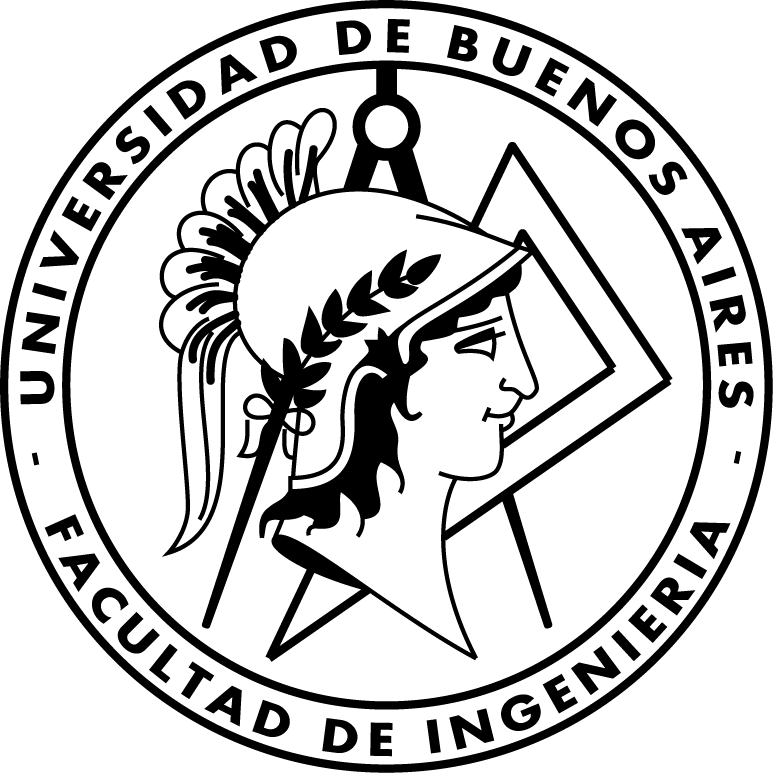
\includegraphics[scale=0.8]{images/logo-fiuba.png} \\
	\begin{center}
		\textbf{Trabajo Práctico N$^{\circ}$3} \linebreak
	\end{center}
	\begin{center}
		\begin{large}
			75.29 - Teoría de Algoritmos I \linebreak
			Facultad de Ingeniería de la Universidad de Buenos Aires \linebreak
			1er. Cuatrimestre 2017 \linebreak
		\end{large}
	\end{center} 
}
\author{	Federico Brasburg, \textit{Padrón Nro. 96.653} \\
			\texttt{ federico.brasburg.@gmail.com } \\ [2.5ex]
			Pablo Rodrigo Ciruzzi, \textit{Padrón Nro. 95.748} \\
			\texttt{ p.ciruzzi@hotmail.com } \\ [2.5ex]
			Andrés Otero, \textit{Padrón Nro. 96.604 } \\
			\texttt{ oteroandres95@gmail.com } \\ [2.5ex] \\
\\
		}
\date{23 de junio de 2017}

\maketitle
\thispagestyle{empty}

\pagebreak 

\tableofcontents
\pagebreak

\clearpage
\section{Programación Dinámica}


\subsection{Cómo correrlo}


\section{Algoritmos Randomizados}
La idea del algoritmo de contracción de Karger es encontrar el corte mínimo en un grafo $G=(V,E)$. Esto es, dos conjuntos no vacíos $A$ y $B$, donde $A \cap B = \varnothing$ y $A \cup B = V$. El tamaño del corte $(A,B)$ se define como el número de aristas $e = (u,v)$ con $u \in A$ y $v \in B$, o viceversa y lo que se busca es que éste sea mínimo.

Este algoritmo es un caso de randomización de tipo \textbf{Monte Carlo}, ya que tiene una probabilidad de que el mismo falle en encontrar la solución correcta.

El algoritmo de contracción en sí consiste en elegir una arista $e=(u,v)$ al azar, y “fusionar” los vértices creando un \textit{supernodo}, el cual tiene tiene todas las aristas de $u$ y $v$ (Salvo la arista entre ellos). Es importante recalcar que el grafo debe permitir múltiples aristas entre dos vértices, ya que al fusionar es importante que se mantengan la cantidad de aristas (Nuevamente, salvo la que es entre $u$ y $v$). Este proceso se debe repetir hasta que el grafo sólo conste de 2 vértices (Notar que en cada ``iteración'' eliminamos un nodo), los cuales se corresponderán con el corte $(A,B)$, y la cantidad de aristas en el grafo será el tamaño del mismo.

Lo más interesante de esto es que su probabilidad de falla es relativamente alta, pero puede ser reducida ampliamente mediante múltiples (en cantidad polinomial) corridas. Yendo a los números, la probabilidad de que el algoritmo sea correcto con una única corrida es de al menos ${\binom{n}{2}}^{-1}$ (con $n = |V|$), lo cual para un $n$ grande es un número muy chico (Es decir, su probabilidad de falla es como mucho $1 - {\binom{n}{2}}^{-1}$). Pero si el mismo se corre $\binom{n}{2}$ veces, se reduce a que se puede fallar en encontrar el corte mínimo con una probabilidad $(1 - {\binom{n}{2}}^{-1})^{\binom{n}{2}} \leq \frac{1}{e}$. Aún más, si se corre $\binom{n}{2}*\ln n$ veces, esta probabilidad desciende a $e^{-\ln n} = \frac{1}{n}$, lo cual es más que aceptable para un $n$ grande.

\subsection{Cómo correrlo}
Correr el algoritmo con una instancia del grafo con $n$ vértices y $2*n$ aristas es tan simple como correr \texttt{python karger.py n} desde la carpeta \texttt{src} del proyecto.

\section{Algoritmos Aproximados}


\subsection{Cómo correrlo}


\pagebreak

\newpage
\section{Código}
\lstset{
	language=Python, columns=flexible, breaklines=true, frame=single, title=creador\_grafos.py
}
\lstinputlisting{../src/creador_grafos.py}

\lstset{ title=grafo.py }
\lstinputlisting{../src/grafo.py}

\lstset{ title=karger.py }
\lstinputlisting{../src/karger.py}

\lstset{ title=parser.py }
\lstinputlisting{../src/parser.py}

\lstset{ title=pg.py }
\lstinputlisting{../src/pg.py}

\lstset{ title=pg\_test.py }
\lstinputlisting{../src/pg_test.py}

\lstset{ title=subset\_sum.py }
\lstinputlisting{../src/subset_sum.py}

\lstset{ title=subset\_sum\_test.py }
\lstinputlisting{../src/subset_sum_test.py}

\end{document}